\documentclass[12pt]{article}

% Packages
\usepackage[margin=0.6in]{geometry}
\usepackage{graphicx}
\usepackage{amsmath}
\usepackage{float}
\usepackage[dvipsnames]{xcolor}
\usepackage{etoolbox}
\usepackage{soul}
%\usepackage{tcolorbox}
%\definecolor{block-gray}{gray}{0.85}

\pagestyle{plain}


\begin{document}

\title{Solution ark \#4.\\ Cluster sampling (one-stage, two-stage)}
\author{O\u{g}uz--Alper, Melike \& Pekarskaya, Tatsiana, Statistics Norway}
\maketitle
\section*{Exercise 0}
Discuss:
\begin{itemize}
\item What is the difference between stratified and cluster samples?\\
\fcolorbox{black}{ForestGreen!20}{
\begin{minipage}[t]{0.97\linewidth}
\textbf{Solution:}
``\textit{Stratified sample:} is a probability sample in which population units are partitioned into strata, and then probability sample of units is taken from each stratum.\\
\textit{Cluster sample:} A probability sample in which each population unit belongs to a group, or cluster, and the clusters are sampled according to the sampling design."\hfill{Lohr, 2019, p.60}
\begin{figure}[H]
\begin{center}
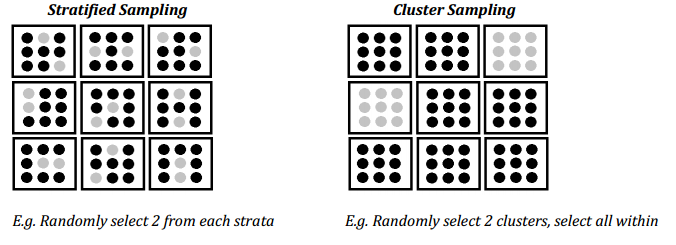
\includegraphics[scale=0.7]{Ex0_1.png}
\end{center}
\end{figure}
Source of the figure: https://medium.com/@pkuaaron/different-sampling-methods-and-their-pros-and-cons-6261b21e7c3a\end{minipage}}
\item What is the difference between one-stage and two-stage sampling?\\
\fcolorbox{black}{ForestGreen!20}{
\begin{minipage}[t]{0.97\linewidth}
\textbf{Solution:}
\textit{One-stage cluster sampling} is a cluster sampling design in which all elements within a sampled cluster are included in the sample. \textit{Two-stage cluster sampling} is a sampling design in which only some elements of selected clusters will be subsampled.
\begin{figure}[H]
\begin{center}
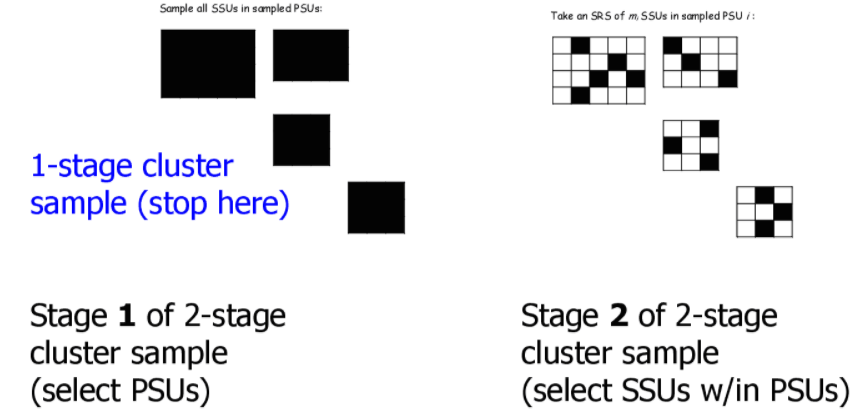
\includegraphics[scale=0.9]{Ex0_2.png}
\end{center}
\end{figure}
Source of the figure: https://www.docsity.com/en/2-stage-cluster-sampling-survey-sampling-techniques-lecture-slides/394133/
\end{minipage}}
\end{itemize}

\section*{Exercise 1}
Kleppel et al. (2004) report on a study of wetlands in upstate New York. Four wetlands
were selected for the study: Two of the wetlands drain watersheds from small towns
and the other two drain suburban watersheds. Quantities such as pH were measured
at two to four randomly selected sites within each of the four wetlands. 
\begin{enumerate}
\item Describe why this is a cluster sample. What are the psus? The ssus? How would you estimate the average pH in the suburban wetlands?\\
\fcolorbox{black}{ForestGreen!20}{
\begin{minipage}[t]{0.97\linewidth}
\textbf{Solution:}
This is a cluster sampling as there are two levels of sampling units: 
\begin{itemize}
\item The wetlands are the PSUs (Primary sampling unit: the unit which is sampled from the population)
\item The sites are the SSUs (Secondary sampling unit: a subunit that is subsampled from the selected psus)
\item The average pH in the suburban wetlands can be estimated by
$$\hat{\bar{Y}}_{sub}=\frac{N_{sub}\sum_{i \in S_{sub}}\hat{t}_{sub;i} /2}{M_{sub;0}},\quad n_{sub}=2,$$
where $\hat{t}_{sub;i}=M_{sub;i}\sum_{j \in S_{sub;i}} y_{sub;ij}/m_{sub;i}$ and $M_{sub;0}=\sum_{i \in U_{sub}}M_{sub;i}$.
\end{itemize}
\end{minipage}}
\item The authors used Student’s two-sample t test to compare the average pH from the sites in the suburban wetlands with the average pH from the sites in the small town wetlands, treating all sites as independent. Is this analysis appropriate? Why, or why not? \\
\fcolorbox{black}{ForestGreen!20}{
\begin{minipage}[t]{0.97\linewidth}
\textbf{Solution:}
Student's two-sample t test assumes that all observations are independent. However, as explained in (1), we have a cluster sample here, and thus, sites within the same wetland are more likely to be similar than sites selected at random from the population. Therefore, the assumption of independence would not be appropriate.
%https://www.datanovia.com/en/lessons/t-test-assumptions/independent-t-test-assumptions/
\end{minipage}}
\end{enumerate}

\section*{Exercise 2}
A city council of a small city wants to know the proportion of eligible voters that
oppose having a incinerator of Phoenix garbage opened just outside of the city limits.
They randomly select $100$ residential numbers from the city’s telephone book that contains $3\,000$ such numbers. Each selected residence is then called and asked for (a) the total number of eligible voters and (b) the number of voters opposed to the incinerator. A total of $157$ voters were surveyed; of these, $23$ refused to answer the question. Of the remaining $134$ voters, $112$ opposed the incinerator, so the council estimates the proportion by
$$\hat{p}=112/134=0.83582$$
with 
$$\hat{V}(\hat{p})=0.83582(1-0.83582)/134=0.00102$$
Are these estimates valid? Why, or why not?\\
\fcolorbox{black}{ForestGreen!20}{
\begin{minipage}[t]{0.97\linewidth}
\textbf{Solution:}
A random sample of $n=100$ residential telephone numbers from $N=3\,000$ such numbers in a city. $157$ voters surveyed and $23$ refused to answer. $112$ voters among $134$ opposed to the incinerator.
\begin{itemize}
\item Assuming non-response is ignorable, $\hat{p}=112/134=0.83582$ is a the ratio estimate of the proportion, and $\hat{p}$ is a consistent estimator of the proportion.
\item  The variance estimator provided is valid for an SRS of $134$ voters. Note that the sampling unit is the residential telephone number, not an individual voter. Therefore, this variance estimator would probably underestimate the true variance, as individuals in the same households are more likely to have similar opinions.  
\end{itemize}
\end{minipage}} 

\section*{Exercise 3}
\textbf{\color{ForestGreen}(R code available)} The new candy Green Globules is being test-marketed in an area of upstate New York. The market research firm decided to sample $6$ cities from the $45$ cities in the area and  then to sample supermarkets within cities, wanting to know the number of cases of
Green Globules sold.
\begin{center}
\begin{tabular}{rrl}
 & Number of &  \\
City& supermarkets & Number of cases sold \\
\hline
1& 52& 146, 180, 251, 152, 72, 181, 171, 361, 73, 186 \\
2& 19& 99, 101, 52, 121\\
3 &37& 199, 179, 98, 63, 126, 87, 62\\
4 &39& 226, 129, 57, 46, 86, 43, 85, 165\\
5 &8 &12, 23\\
6 &14 &87, 43, 59\\
\end{tabular}
\end{center}
Obtain summary statistics for each cluster. Plot the data, and estimate the total number of cases sold, and the average number sold per supermarket, along with the standard errors of your estimates. \hfill (Lohr, 2019, p.209)\\
\fcolorbox{black}{ForestGreen!20}{
\begin{minipage}[t]{0.97\linewidth}
\textbf{Solution:}
$n=6$ cities are sampled from $N=45$ cities. For each city, a random sample of supermarkets is taken.
\begin{figure}[H]
\begin{center}
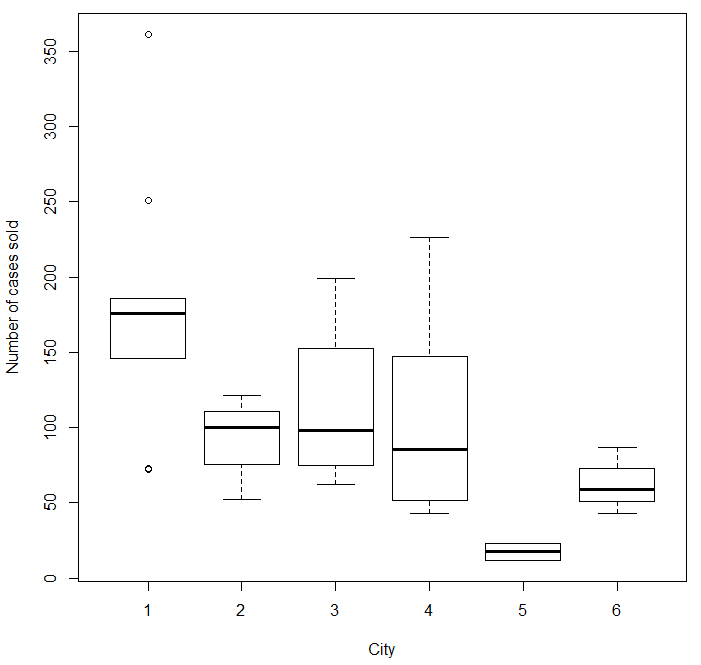
\includegraphics[scale=0.8]{Ex3.png}
\end{center}
\end{figure}
\begin{center}
\begin{tabular}{rrrrrrr}
$i\in S$ & $M_i$ & $m_i$ & \multicolumn{1}{c}{$\bar{y}_i$} & \multicolumn{1}{c}{$s_i$} & \multicolumn{1}{c}{$\hat{t}_i$} & $M_i^2(1-m_i/M_i)s_i^2/m_i$\\        
\hline
1& 52& 10 & 177.30 &83.5996 & 9 219.60 &1 526 376 \\
2& 19& 4 & 93.25& 29.2390 & 1 771.75 &60 913\\
3 &37& 7 & 116.29&54.5396 & 4 302.57&471 682 \\
4 &39& 8 & 104.62&64.5931 & 4 080.38 & 630 534\\
5 &8 &2 & 17.50& 7.7782&140.00 & 1 452\\
6 &14 &3 & 63.00&22.2711 & 882.00 & 25 461\\
\hline
Sum & 169 & 34 & & & 20 396.26 & 2 716 418\\
\end{tabular}
\end{center}
Here, $\hat{t}_i=M_i\sum_{j \in S_i}y_{ij}/m_i= M_i\bar{y}_i$. Using $$\hat{t}=\frac{N}{n}\sum_{i \in S} \hat{t}_i=\frac{45}{6}\sum_{i \in S} \hat{t}_i,$$ 
we obtain
$$\hat{t}=7.5*(9\,219.6+1\,771.75+\cdots+882)=152\,972.2$$
\end{minipage}}\\
\fcolorbox{black}{ForestGreen!20}{
\begin{minipage}[t]{0.97\linewidth}
To estimate the average number of cases sold per supermarket, we can use
$$\hat{\bar{Y}}_r=\frac{\hat{t}}{\hat{M}_0}=\frac{\sum_{i \in S}\hat{t}_i}{\sum_{i \in S}M_i}, \quad \hat{t}=\frac{N}{n}\sum_{i \in S}\hat{t}_i, \, \hat{M}_0=\frac{N}{n}\sum_{i \in S}M_i$$
Here, $\hat{\bar{Y}}_r$ is a ratio estimator of the population mean, where $M_i$ is the auxiliary variable. Thus, we find
$$\hat{\bar{Y}}_r=\frac{20\,396.26}{169}=120.69$$

The variance of $\hat{t}$ under a two-stage cluster sampling can be estimated by 
$$\hat{V}(\hat{t})=N^2\Big(1-\frac{n}{N}\Big)\frac{s_t^2}{n}+\frac{N}{n}\sum_{i\in S}M_i^2\Big(1-\frac{m_i}{M_i}\Big)\frac{s_i^2}{m_i},$$
where 

$$s_t^2=\frac{1}{n-1}\sum_{i \in S}\Big(\hat{t}_i-\frac{\hat{t}}{N}\Big)^2=\frac{1}{n-1}\sum_{i \in S}\Big(\hat{t}_i-\frac{\sum_{i \in S}\hat{t}_i}{n}\Big)^2$$
\begin{eqnarray*}
\widehat{SE(\hat{t})}&=&\sqrt{45^2\Big(1-\frac{6}{45}\Big)\frac{10\,952\,882}{6}+\frac{45}{6}2\,716\,418}\\
&=& \sqrt{3\,203\,717\,942+20\,373\,134} = \sqrt{3\,224\,091\,076} = 56\,781
\end{eqnarray*}
The variance of $\hat{\bar{Y}}_r=\hat{t}/(N\bar{m})$, with $\bar{m}=\sum_{i\in S}M_i/n$, can be estimated by
\begin{eqnarray*}
\hat{V}(\hat{\bar{Y}}_r)&=&\frac{1}{\bar{m}^2}\Big(1-\frac{n}{N}\Big)\frac{s_e^2}{n}+\frac{1}{nN\bar{m}^2}\sum_{i\in S}M_i^2\Big(1-\frac{m_i}{M_i}\Big)\frac{s_i^2}{m_i} \\
&=&\frac{1}{28.17^2}\Big(1-\frac{6}{45}\Big)\frac{2\,138\,111}{6}+\frac{1}{6(45)28.17^2}2\,716\,418\\
&=& 389.28+12.68=401.96,
\end{eqnarray*}
where 
$$s_e^2=\frac{1}{n-1}\sum_{i \in S}(e_i-\bar{e})^2=\frac{1}{n-1}\sum_{i \in S}M_i^2(\bar{y}_i-\hat{\bar{Y}}_r)^2,\quad e_i=\hat{t}_i-M_i\hat{\bar{Y}}_r,\, \bar{e}=0\cdot$$
Thus, we have $\widehat{SE}(\bar{y}_r)=\sqrt{\hat{V}(\bar{y}_r)}=\sqrt{401.96}=20.05$.

\end{minipage}}

\section*{Exercise 4}
An accounting firm is interested in estimating the error rate in a compliance audit it is
conducting. The population contains $828$ claims, and the firm audits an SRS of $85$ of
those claims. In each of the $85$ sampled claims, $215$ fields are checked for errors. One
claim has errors in $4$ of the $215$ fields, $1$ claim has $3$ errors, $4$ claims have $2$ errors,
$22$ claims have $1$ error, and the remaining $57$ claims have no errors. (Data courtesy of
Fritz Scheuren.)
\begin{enumerate}
\item Treating the claims as psus and the observations for each field as ssus, estimate the error rate, defined to be the average number of errors per field, along with the standard error for your estimate.\\
\fcolorbox{black}{ForestGreen!20}{
\begin{minipage}[t]{0.97\linewidth}
\textbf{Solution:}

This is a one-stage cluster sampling, and so $\pi_{j|i}=1$. 
\begin{eqnarray*}
\hat{t}&=&\frac{828}{85}\sum_{i \in S}t_i, \quad t_i=0,1,2,3,4 \\
&=&\frac{828}{85}\Big[57(0)+22(1)+4(2)+1(3)+1(4)\Big] \\
&=&\frac{828}{85}(37)=360.42\cdot
\end{eqnarray*}
Thus the error rate is found by
$$\bar{y}=\frac{\hat{t}}{NM}=\frac{360.42}{(828)(215)}=0.002025\cdot$$
Note that $\bar{y}$ is an unbiased estimator of the population mean unlike the one used in Exercise 3, where denominator of the ratio was random. \\The standard error of $\bar{y}$ is obtained using
\begin{eqnarray*}
\widehat{SE}(\bar{y})&=&\sqrt{\frac{1}{M^2}\Big(1-\frac{n}{N}\Big)\frac{s_t^2}{n}} \\
&=&\frac{1}{215}\sqrt{\Big(1-\frac{85}{828}\Big)\frac{s_t^2}{85}}\\
&=&\frac{1}{215}(0.07677)\\
&=&0.000357,
\end{eqnarray*}
where
\begin{eqnarray*}
s_t^2&=&\frac{1}{84}\sum_{i \in S}\Big(t_i-\frac{\sum_{i \in S}t_i}{n}\Big)^2\\
&=&\frac{1}{84}\Big[57\Big(0-\frac{37}{85}\Big)^2 + 22\Big(1-\frac{37}{85}\Big)^2 + \cdots + 1\Big(4-\frac{37}{85}\Big)^2\Big] \\
&=& \frac{1}{84}(10.80+7.02+9.79+6.58+12.71)\\
&=& 0.5583 
\end{eqnarray*}

\end{minipage}}
\item Estimate (with standard error) the total number of errors in the $828$ claims.\\
\fcolorbox{black}{ForestGreen!20}{
\begin{minipage}[t]{0.97\linewidth}
\textbf{Solution:}
We have $\hat{t}=360.42$ from (1). The standard error of $\hat{t}$ can be found by 
\begin{eqnarray*}
\widehat{SE}(\hat{t})&=&\sqrt{N^2\Big(1-\frac{n}{N}\Big)\frac{s_t^2}{n}} \\
&=&828\sqrt{\Big(1-\frac{85}{828}\Big)\frac{s_t^2}{85}}\\
&=&828(0.07677) = 63.5656
\end{eqnarray*}

\end{minipage}}
\item Suppose that instead of taking a cluster sample, the firm had taken an SRS of $85\times 215=18\,275$ fields from the $178\,020$ fields in the population. If the estimated
error rate from the SRS had been the same as in (1), what would the estimated
variance $\hat{V}(\hat{p}_{srs})$ be? How does this compare with the estimated variance
from (1)?\\
\fcolorbox{black}{ForestGreen!20}{
\begin{minipage}[t]{0.97\linewidth}
\textbf{Solution:}
Suppose we have an SRS sample of $n=85\times 215=18\,275$ fields from a total of $N=178\,020$ fields. Assume the same error rate found in (a), that is, $\hat{p}_{srs}=\bar{y}=0.002025$. Find $\hat{V}(\hat{p}_{srs})$.
\begin{eqnarray*}
\hat{V}(\hat{p}_{srs})&=&\Big(1-\frac{n}{N}\Big)\frac{\hat{p}_{srs}(1-\hat{p}_{srs})}{n-1}\\
&=& \Big(1-\frac{18\,275}{178\,020}\Big)\frac{0.002025(0.997975)}{18\,275}\\
&=&9.92\times 10^{-8}\cdot
\end{eqnarray*}
The estimated variance under cluster design is $\hat{V}(\bar{y})=SE(\bar{y})^2=1.28\times 10^{-7}$. Thus, the ratio of variances is
$$\frac{\hat{V}(\bar{y})}{\hat{V}(\hat{p}_{srs})}=\frac{1.27\times 10^{-7}}{9.92\times 10^{-8}}=1.28\cdot$$
\end{minipage}}
\end{enumerate}

\section*{Exercise 5}
\textbf{\color{ForestGreen}(R code available)} The file measles.dat contains data consistent with that obtained in a survey of parents
whose children had not been immunized for measles during a recent campaign to
immunize all children between the ages of $11$ and $15$. During the campaign, $7\,633$ children
from the $46$ schools in the area were immunized; $9\,962$ children whose records
showed no previous immunization were not immunized. In a follow-up survey to
explore why the children had not been immunized during the campaign, Roberts
et al. (1995) sent questionnaires to the parents of a cluster sample of the $9\,962$ children.
Ten schools were randomly selected, then a sample of the $m_i$ nonimmunized
children from each school was selected and the parents of those children were sent a
questionnaire.
\begin{enumerate}
\item Estimate, separately for each school, the percentage of parents who returned a consent form (variable \emph{returnf}). For this exercise, treat the “no answer” responses (value 9) as not returned.\\
\fcolorbox{black}{ForestGreen!20}{
\begin{minipage}[t]{0.97\linewidth}
\textbf{Solution:}
We use variables \emph{form} and \emph{returnf}. The former is used to find the total number of parents received a consent form, that is $k_i$.
\begin{center}
\begin{tabular}{rrrrrrr}
School & $M_i$ & $m_i$ & $k_i$ & Return &$\bar{y}_i$ & $\hat{t}_i$ \\    
\hline
1 & 78 &40 &38 &19 &0.5000& 39.000\\
2 &238 &38 &36& 19& 0.5278&125.611\\
3&261& 19 &17& 13 &0.7647&199.588\\
4 &174 &30& 30 &18& 0.6000&104.400\\
5 &236 &30 &26& 12 &0.4615&108.923\\
6 &188& 25 &24& 13& 0.5416&101.833\\
7& 113& 23& 22& 15& 0.6818&77.045\\
8& 170 &43& 36 &21& 0.5833&99.167\\
9 &296 &38& 35 &23& 0.6571&194.514\\
10& 207 &21& 17&  7& 0.4118&85.235\\
\hline
Sum & 1 961 & 307&281&160&& 1 135.317\\
\end{tabular}
\end{center}

\end{minipage}}
\item Using the number of respondents in school $i$ as $m_i$, construct the sampling weight for each observation.\\
\fcolorbox{black}{ForestGreen!20}{
\begin{minipage}[t]{0.97\linewidth}
\textbf{Solution:}

Treating $k_i$ as $m_i$, the sampling weight for each observation is given by
$$w_{ij}=w_i w_{j|i}=\frac{N}{n}\frac{M_i}{k_i}=\frac{46}{10}\frac{M_i}{k_i},$$
where $M_i/k_i=2.05,6.61, 15.35,  5.80,  9.08,  7.83,  5.14,  4.72,  8.46,12.18$, for $i=1,2,3,4,5,6,7,8,9,10$, respectively.\\

\end{minipage}}
\item Estimate the overall percentage of parents who received a consent form along with a $95\%$ CI.\\
\fcolorbox{black}{ForestGreen!20}{
\begin{minipage}[t]{0.97\linewidth}
\textbf{Solution:}
Estimate $\bar{Y}$ and give a $95\%$ CI for your estimate.
$$\hat{\bar{Y}}_r=\frac{\sum_{i \in S}\hat{t}_i}{\sum_{i \in S}M_i}=\frac{1\,135.317}{1\,961}=0.5789\cdot$$
\begin{eqnarray*}
\widehat{SE}(\hat{\bar{Y}}_r)&=&\frac{1}{196.1}\sqrt{\Big( 1-\frac{10}{46}\Big)\frac{s_e^2}{10} + \frac{1}{10(46)}\sum_{i\in S}M_i^2\Big(1-\frac{k_i}{M_i}\Big)\frac{s_i^2}{k_i}}\\
&=&\frac{1}{196.1}\sqrt{\Big( 1-\frac{10}{46}\Big)\frac{581.797}{10} + \frac{1}{10(46)}3\,484.187}\\
&=&\frac{1}{196.1}\sqrt{45.532 + 7.574} = 0.03716\cdot
\end{eqnarray*}
Thus, an approximate $95\%$ CI is given by 
\vspace{-0.2cm}
$$0.5789\pm 1.96(0.0372)=[0.5061,0.6518]\cdot$$


\end{minipage}}
\item How do your estimate and interval in part (3) compare with the results you would have obtained if you had ignored the clustering and analyzed the data as an SRS?
Find the ratio:
\begin{center}
\begin{tabular}{c}
estimated variance from (3) \\
\hline
estimated variance if the data were analyzed as an SRS  \\
\end{tabular}
\end{center}
What is the effect of clustering? \\
\fcolorbox{black}{ForestGreen!20}{
\begin{minipage}[t]{0.97\linewidth}
\textbf{Solution:}
Ignoring clustering and assuming as if the observations came from an SRS sample, we would have
$$\hat{p}_{srs}=\frac{160}{281}=0.5694,$$
$$\hat{V}(\hat{p}_{srs})=\frac{0.5694(1-0.5694)}{280}=0.000876\cdot$$
The effect of clustering can be found by
$$\widehat{DEFF} = \frac{\hat{V}_{scs}(\hat{\bar{Y}}_r)}{\hat{V}(\hat{p}_{srs})}=\frac{0.03716^2}{0.000876}=\frac{0.001381}{0.000876}=1.58\cdot$$


\end{minipage}}
\end{enumerate}

\end{document}